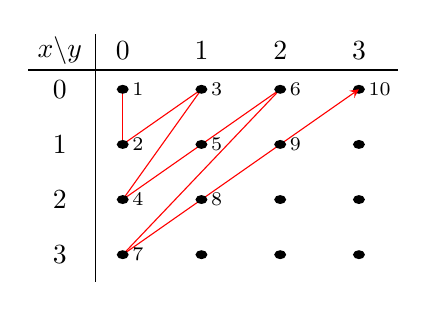
\begin{tikzpicture}[yscale=.7]
			\usetikzlibrary{arrows.meta}
			
			\tikzset{
				myarrow/.style=-stealth
			}
			
			\foreach \x in {0,1,2,3} {
				\node at (.2,-\x-1) {\x};
			}
			\foreach \y in {0,1,2,3} {
				\node at (\y+1,-.3) {\y};
			}
			\draw[red] (1,-1) -- (1,-2);
			\draw[red] (1,-2) -- (2,-1);
			\draw[red] (2,-1) -- (1,-3);
			\draw[red] (1,-3) -- (3,-1);
			\draw[red] (3,-1) -- (1,-4);
			\draw[red] (1,-4) -- (3+.2,-2+.2);
			
			\node at (.2,-.3) {$x\backslash y$};
			\foreach \x in {0,1,2,3} {
				\foreach \y in {0,1,2,3} {
					\ifthenelse{\x<\y \OR \x=\y}{
						\draw[thick,fill] (4-\y,-\x-1) circle (.06);
					}{}
				}
			}
			\draw[myarrow,red] (3+.2,-2+.2) -- (4,-1);
			\node[right] at (1,-1) {\scriptsize 1};
			\node[right] at (1,-2) {\scriptsize 2};
			\node[right] at (2,-1) {\scriptsize 3};
			\node[right] at (1,-3) {\scriptsize 4};
			\node[right] at (2,-2) {\scriptsize 5};
			\node[right] at (3,-1) {\scriptsize 6};
			\node[right] at (1,-4) {\scriptsize 7};
			\node[right] at (2,-3) {\scriptsize 8};
			\node[right] at (3,-2) {\scriptsize 9};
			\node[right] at (4,-1) {\scriptsize 10};
			
			\draw (-.2,-.65) -- (4.5,-.65);
			\draw (.65,0) -- (.65,-4.5);
			
\end{tikzpicture}
